\documentclass{article}
\usepackage{parskip}
\usepackage{amsmath}
\usepackage[dvipdfmx]{graphicx}
\begin{document}

点$(sx, sy), (tx, ty)$をそれぞれ$S, T$とおき,
$\Delta x = tx - sx,\ \Delta y = ty - sy$とおく。
$S, T$を除き同じ座標を複数回通らないという制約により,
求める最短経路は$S$に隣接する4点と$T$に隣接する4点をすべて1回ずつ通る。

$S$に隣接する点のひとつを$S_1$とおき,
それ以外を$S$を中心に反時計回りに$S_2, S_3, S_4$とおく。
さらに,$T$に隣接する点のひとつを選んで$S_1$と線で結ぶ。
選んだ点を$T_1$とおき,それ以外を$T$を中心に時計回りに$T_2, T_3, T_4$とおく(\ref{g1})。

\begin{figure}[h]
    \begin{center}
        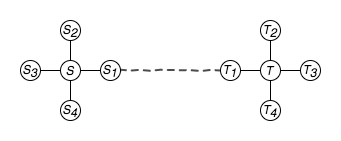
\includegraphics[width=250pt]{fig1.png}
        \caption{$S_1$と結んだ点を$T_1$とおく}
        \label{g1}
    \end{center}
\end{figure}

このとき,他の点同士の結び方は$3 \times 3 = 9$通りあるが,
このうち線同士が交差しないような結び方は,互いに同じ番号の点同士を結ぶ場合に限られる(\ref{g2})。
% もう少し厳密に証明したい

\begin{figure}[h]
    \begin{center}
        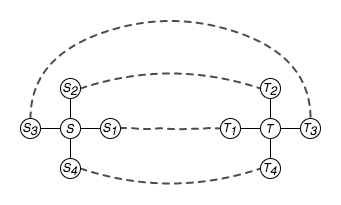
\includegraphics[width=250pt]{fig2.png}
        \caption{互いに同じ番号の点同士を結ぶ}
        \label{g2}
    \end{center}
\end{figure}

したがって,点$(sx + 1, sy)$を$S_1$とおくことにすれば,
経路の選び方は座標平面上で$T_1$を$T$の上下左右どこにとるかによって4通りに場合分けされる。

ここで,互いに結んだ2点間の最短経路の長さは2点間のマンハッタン距離を下回ることはないので,
4通りのいずれに対しても,最短経路の長さ$d$に関する次の不等式が成り立つ:
\begin{equation*}
    d \geq 4 (\Delta x + \Delta y) + 8
\end{equation*}

したがって,最短経路の長さが$4 (\Delta x + \Delta y) + 8$であるような経路で,
かつ$S, T$を除き同じ座標を複数回通ることがないようなものが存在するならば,
それは求める最短経路のひとつであるが,次のような経路はこの条件を満たす:
\begin{quote}
    i) $S$から$\Delta x$だけ右,$\Delta y$だけ上に進んで$T$に着く \\
    ii) $T$から$\Delta x$だけ左,$\Delta y$だけ下に進んで$S$に着く \\
    ii) $S$から1だけ左,$\Delta y + 1$だけ上,$\Delta x + 1$だけ右,1だけ下に進んで$T$に着く \\
    ii) $T$から1だけ右,$\Delta y + 1$だけ下,$\Delta x + 1$だけ左,1だけ上に進んで$S$に着く
\end{quote}

\end{document}
